\chapter{BPMN Notation}


\begin{figure}[!htbp]
\begin{center}
  \includegraphics[width=\linewidth]{BPM} %pdf, jpg, png...
  \caption{BPMN Ereignisse}
  \label{fig:BPM}
\end{center}
\end{figure}

\begin{figure}[!htbp]
\begin{center}
  \includegraphics[width=\linewidth]{BPM_2} %pdf, jpg, png...
  \caption{BPMN Übersicht}
  \label{fig:BPM_2}
\end{center}
\end{figure}

\begin{figure}[!htbp]
\begin{center}
  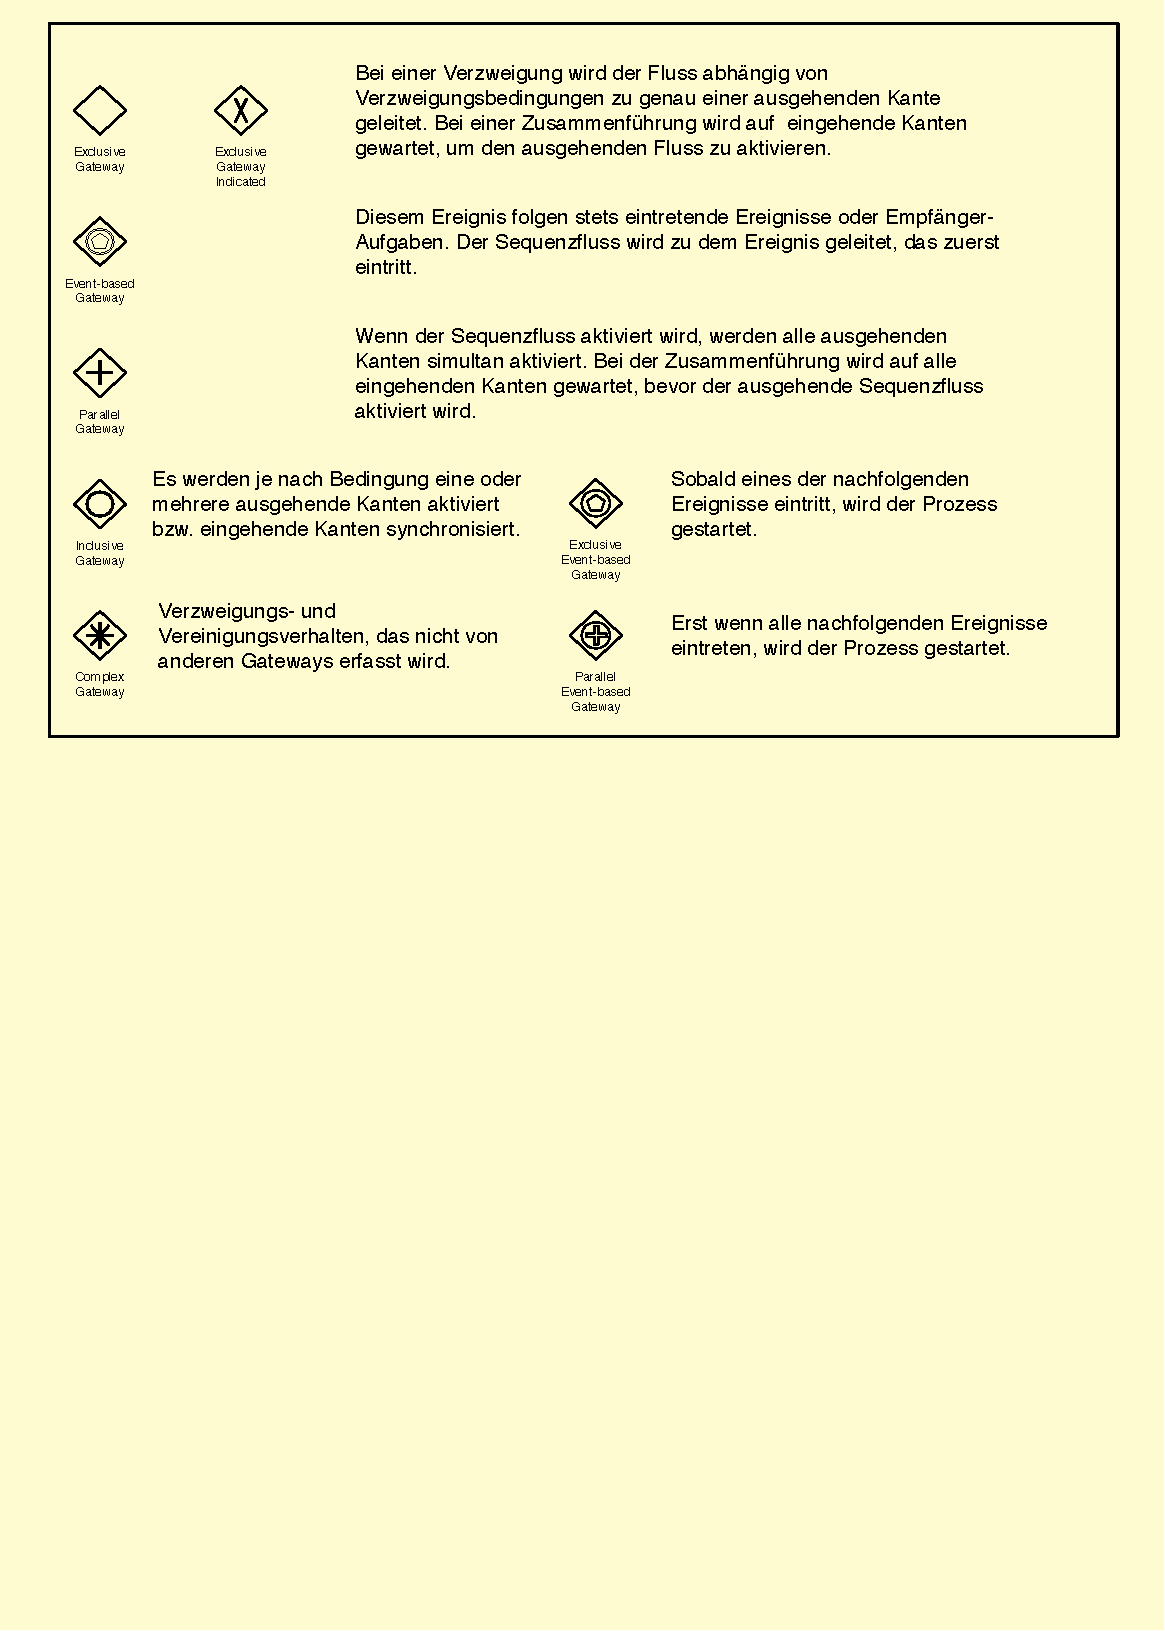
\includegraphics[width=\linewidth]{gatewa} %pdf, jpg, png...
  \caption{BPMN Gateways}
  \label{fig:gateways}
\end{center}
\end{figure}

\chapter{ConDec Notation}

 
 
 \begin{table}[H]
 \begin{tabular}{|p{0.5\textwidth}|p{0.5\textwidth}|}
\hline
\textbf{Notation} & \textbf{Erläuterung}\\
\hline
\begin{center}
  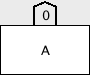
\includegraphics[scale=0.5]{absence} %pdf, jpg, png...
  \end{center}
& \textbf{absence (A)} \newline
Aktivität A darf nicht ausgeführt werden

\\



\hline
\begin{center}

  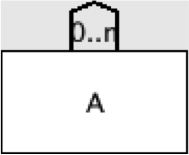
\includegraphics[scale=0.5]{absenceN} %pdf, jpg, png...
    \end{center}

& \textbf{absence (n+1, A)} \newline
Aktivität A kann höchsten n mal ausgeführt werden, aber nicht n+1-mal

\\
\hline
\begin{center}

  \includegraphics[scale=0.5]{existenceN} %pdf, jpg, png...
    \end{center}

& \textbf{existence (n, A)}\newline
Aktivität A muss mindestens n-mal ausgeführt werden

\\
\hline
\begin{center}

  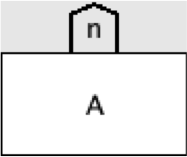
\includegraphics[scale=0.5]{ExactlyN} %pdf, jpg, png...
    \end{center}

& \textbf{exactly (n, A)}\newline
Aktivität A muss genau n-mal ausgeführt werden ausgeführt werden

\\
\hline

\begin{center}

  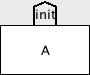
\includegraphics[scale=0.5]{Init} %pdf, jpg, png...
    \end{center}

& \textbf{init (A)}\newline
Aktivität A muss als erste Aktivität ausgeführt werden

\\
\hline

\end{tabular}
 \caption{ExistenceConstraints ConDec}
\label{tab:existence}
\end{table}

%Tabelle Neu

\begin{tabular}{|p{0.5\textwidth}|p{0.5\textwidth}|}
\hline
\textbf{Constraint} & \textbf{Erläuterung}\\
\hline

\begin{center}

  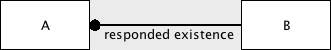
\includegraphics[scale=0.5]{RespondedExistence} %pdf, jpg, png...
    \end{center}&

\textbf{responded existence} \newline  Falls A ausgeführt wird, muss B entweder davor oder danach ebenfalls ausgeführt werden. \newline
Beispiel: Korrekt: [A,B]; [B,A]; Inkorrekt:[A];
\\
\hline
\begin{center}

  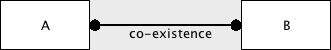
\includegraphics[scale=0.5]{CoExistence} %pdf, jpg, png...
    \end{center} &
\textbf{co-existence} \newline A und B kommen in einem Pfad immer zusammen vor.\newline
Beispiel: Korrekt: [A,B]; Inkorrekt: [A]; [B];
 \\
\hline

\begin{center}

  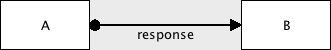
\includegraphics[scale=0.5]{response} %pdf, jpg, png...
    \end{center} &
\textbf{response} \newline Falls A ausgeführt wird, muss B danach ebenfalls ausgeführt werden. \newline
Beispiel: Korrekt: [B,A,A,A,C,B]; Inkorrekt: [B,A,A,A,C]
\\
\hline
\begin{center}

  \includegraphics[scale=0.5]{Precedence} %pdf, jpg, png...
    \end{center} &
    \textbf{precedence}\newline
Falls B  ausgeführt wird, muss vorher A ausgeführt werden. \newline
Beispiel: Korrekt: [A,C,B,B,A]; Inkorrekt:[C,B,B,A]
\\
\hline
\begin{center}

  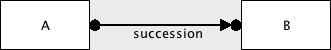
\includegraphics[scale=0.5]{Succession} %pdf, jpg, png...
    \end{center}&
\textbf{succession} \newline Verlangt, dass die beiden Constraints precedence und response zwischen den Aktivitäten A und B eingehalten werden. Somit muss jede Aktivirtät A von Aktivität B gefolgt werden und für jede Aktivität B muss eine Aktivität A vorhanden sein. \newline
Beispiel: Korrekt: [A,C,A,B,B]; Inkorrekt: [A,C,B,B]\\
\hline
 \begin{center}

  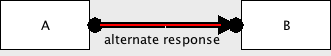
\includegraphics[scale=0.5]{AlternateResponse} %pdf, jpg, png...
    \end{center} &
\textbf{alternate response}  Verlangt, dass nach einer Aktivität A Aktivität B ausgeführt wird, jedoch darf vor Aktivität B nicht eine weiter Aktivität A ausgeführt werden. \newline
Beispiel: Korrekt: [B,A,C,B,A,B] ; Inkorrekt: [B,A,C,A,B,A,B] \\
\hline
\end{tabular}
\begin {table}

\begin{tabular}{|p{0.5\textwidth}|p{0.5\textwidth}|}

\hline
\begin{center}

  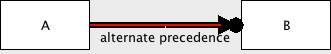
\includegraphics[scale=0.5]{AlternatePrecedence} %pdf, jpg, png...
    \end{center} &
\textbf{alternate precedence}\newline
  Verlangt, dass jeder Instanz von Aktivität B eine Instanz der Aktivität A vorausgeht. Die nächste Instanz einer Aktivität B kann somit nicht vor der nächsten Instanz von Aktivität A ausgeführt werden.
  \newline
  Beispiel: Korrekt: [A,C,B,A,B,A]; Inkorrekt: [A,C,B,B,A]\\
\hline
\begin{center}

  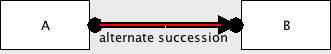
\includegraphics[scale=0.5]{AlternateSuccession} %pdf, jpg, png...
    \end{center}&
\textbf{alternate succession} \newline
 Stellt eine Kombination aus alternate response und alternate precedence dar. \newline
  Beispiel:  Korrekt: [A,C,B,A,B,A,B]; Inkorrekt: [C,B,A,A,B] \\
\hline
\begin{center}

  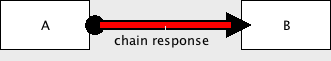
\includegraphics[scale=0.5]{ChainResponse} %pdf, jpg, png...
    \end{center}&
 \textbf{chain response}\newline
  Verlangt, dass die nächste Aktivität, welche nach Aktivität A ausgeführt wird, Aktivität B ist. \newline
  Beispiel: Korrekt: [B,A,B,C,A,B]; Inkorrekt: [B,A,C,A,B]\\
\hline
\begin{center}

  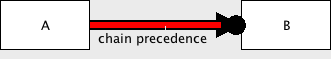
\includegraphics[scale=0.5]{ChainPrecedence} %pdf, jpg, png...
    \end{center}&
\textbf{chain precedence} \newline
 Verlangt, dass Aktivität A unmittelbar bevor Aktivität B ausgeführt wird.\newline
 Beispiel: Korrekt: [A,B,C,A,B,A]; Inkorrekt: [A,B,C,B,A] \\
\hline
\begin{center}

  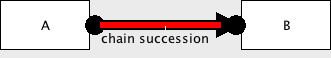
\includegraphics[scale=0.5]{ChainSuccession} %pdf, jpg, png...
    \end{center} &
\textbf{chain succession} \newline  Stellt eine Kombination aus chain response und chain precedence dar und verlangt, dass Aktivität A und Aktivität B jeweils nebeneinander ausgeführt werden. \newline
Beispiel: Korrekt: [A,B,C,A,B,A,B]; Inkorrekt: [A,B,C,A,B,A,B,A,C]\\
\hline
 \end{tabular}
 \caption{Relation Constraints ConDec}
\label{tab:relation}
 \end{table}

 
%Tabelle Neu

\begin{tabular}{|p{0.5\textwidth}|p{0.5\textwidth}|}
\hline
\textbf{Constraint} & \textbf{Erläuterung}\\
\hline

\begin{center}

  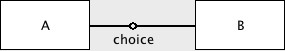
\includegraphics[scale=0.5]{Choice} %pdf, jpg, png...
    \end{center}&

\textbf{choice} \newline  Mindestens eine der beiden Aktivitäten A oder B muss ausgeführt werden.  \newline
Beispiel: Korrekt: [A]; [B]; Inkorrekt:[ ];
\\
\hline

\begin{center}
  \includegraphics[scale=0.5]{ChoiceOneOfThree} %pdf, jpg, png...
    \end{center} &
    \textbf{choice 1 of 3}\newline
Mindestens eine der drei Aktivitäten A,B oder C muss ausgeführt werden.. \newline
Beispiel: Korrekt: [A; Inkorrekt:[]
\\
\hline
\begin{center}

  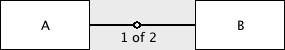
\includegraphics[scale=0.5]{ChoiceOneOfTwo} %pdf, jpg, png...
    \end{center}&
\textbf{1 of 2} \newline Entweder A oder b muss mindestens einmal ausgeführt werden.\newline
Beispiel: Korrekt: [A,C,A,B,B]; Inkorrekt: [A,C,B,B]\\
\hline

\end{tabular}

\begin {table}

\begin{tabular}{|p{0.5\textwidth}|p{0.5\textwidth}|}

\hline
\begin{center}

  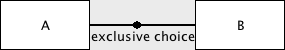
\includegraphics[scale=0.5]{ExclusiveChoice} %pdf, jpg, png...
    \end{center} &
\textbf{alternate precedence}\newline
  Verlangt, dass jeder Instanz von Aktivität B eine Instanz der Aktivität A vorausgeht. Die nächste Instanz einer Aktivität B kann somit nicht vor der nächsten Instanz von Aktivität A ausgeführt werden.
  \newline
  Beispiel: Korrekt: [A,C,B,A,B,A]; Inkorrekt: [A,C,B,B,A]\\
\hline
\begin{center}

  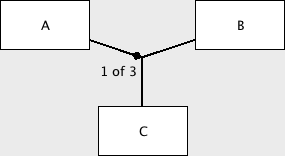
\includegraphics[scale=0.5]{ExclusiveChoiceOneOfThree} %pdf, jpg, png...
    \end{center}&
\textbf{alternate succession} \newline
 Stellt eine Kombination aus alternate response und alternate precedence dar. \newline
  Beispiel:  Korrekt: [A,C,B,A,B,A,B]; Inkorrekt: [C,B,A,A,B] \\
\hline
 \end{tabular}
 \caption{Choice Constraints ConDec}
\label{tab:relation}
 \end{table}
 
 %Neue Tabelle
 
 
 \begin {table}[H]

\begin{tabular}{|p{0.5\textwidth}|p{0.5\textwidth}|}
\hline
\begin{center}

  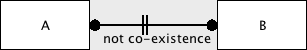
\includegraphics[scale=0.5]{NotCoExistence} %pdf, jpg, png...
    \end{center} &
\textbf{not co-existence}\newline
  Verlangt, dass falls Aktivität A ausgeführt wird, darf Aktivität B nicht mehr ausgeführt werden und umgekehrt.
  \newline
  Beispiel: Korrekt: [A,C,A,A] ; Inkorrekt: [A,C,A,A,B] \\
\hline

\hline
\begin{center}

  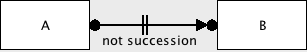
\includegraphics[scale=0.5]{NotSuccession} %pdf, jpg, png...
    \end{center} &
\textbf{not succession}\newline
  Verlangt, dass falls Aktivität A ausgeführt wird, darf Aktivität B nicht danach ausgeführt werden.
  \newline
  Beispiel: Korrekt: [B,B,C,A,C,A,A] ; Inkorrekt: [A,C,B]\\
\hline

\hline
\begin{center}

  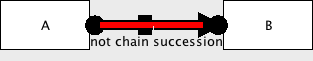
\includegraphics[scale=0.5]{NotChainSuccession} %pdf, jpg, png...
    \end{center} &
\textbf{negation chain succession}\newline
  Verlangt, dass die Aktivitäten A und B nicht nebeneinander ausgeführt werden.
  \newline
  Beispiel: Korrekt: [B,A,C,B,A] ; Inkorrekt: [B,A,B,A] \\
\hline

 \end{tabular}
 \caption{Negotation Constraints ConDec}
\label{tab:relation}
 \end{table}

\cite{Montali2010, Pesic200}
